\chapter{Week 11}

\section{URDF Extension II}

    The URDF Extension was initialized from the JupyterLab extension \textit{cookiecutter} which greatly simplifies the process. Afterwards, the model and widget and their respective factories were created by following the \href{https://github.com/jupyterlab/extension-examples/tree/master/documents}{Documents extension} example. In order to make the widget more accessible, a button to open the viewer was added to the main menu and the launcher page as shown in Figure~\ref{fig:startURDF}. The same command was also included in the command palette. The viewer can also be accessed by double clicking on any \texttt{.urdf} file.

    \begin{figure}[H]
        \centering
        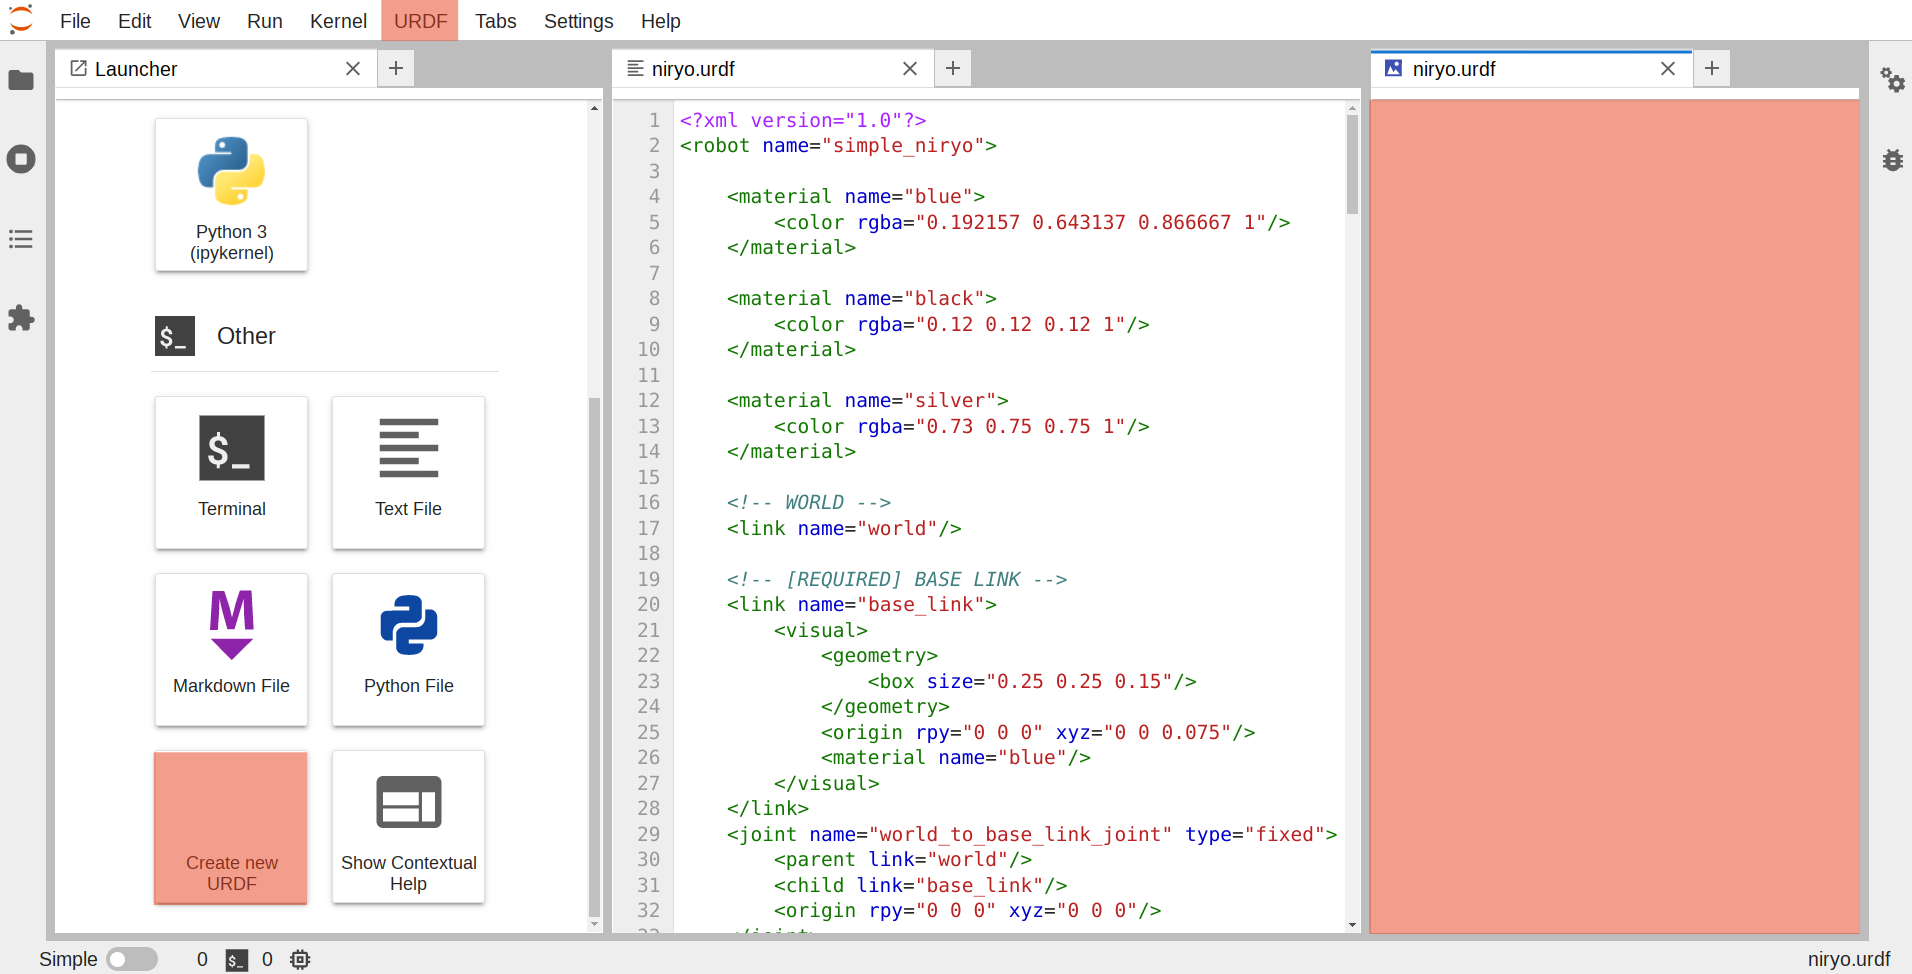
\includegraphics[width=\linewidth]{Images/11_startURDF_red.png}
        \caption{The URDF widget (right) can be accessed from the main menu (top) and the launcher (left).}
        \label{fig:startURDF}
    \end{figure}

    \noindent One of the current issues is that the buttons will only open the URDF viewer widget, but in order to read the file, this needs to be separately opened with a text editor. The current opening command needs to be modified, or another command needs to be added, which will open both a text editor for the XML file and the URDF viewer to display the contents of the file.

    Given that working with URDF's is very common in the robotics community, other developers have already tackled the problem of visualizing the contents of these files. An example of this is the \href{https://github.com/danidask/urdf_editor}{\texttt{urdf\_editor}} observed in Figure~\ref{fig:r2d2}; this example uses the \href{https://p5js.org/}{p5.js} library to sketch all the robot components on a browser canvas. Although this \texttt{urdf\_editor} accomplishes the same goal as what is desired for our extension, the project has mostly been abandoned and has some issues with user interaction.

    Another example is the \href{https://github.com/gkjohnson/urdf-loaders}{\texttt{urdf-loaders}} illustrated in Figure~\ref{fig:johnsonURDF}. One of these loaders uses the \href{https://threejs.org/}{THREE.js} library which is very popular in contemporary visualization applications. And since this loader has been more recently updated, this makes it an ideal choice to integrate into our URDF extension.

    \begin{figure}[H]
        \centering
        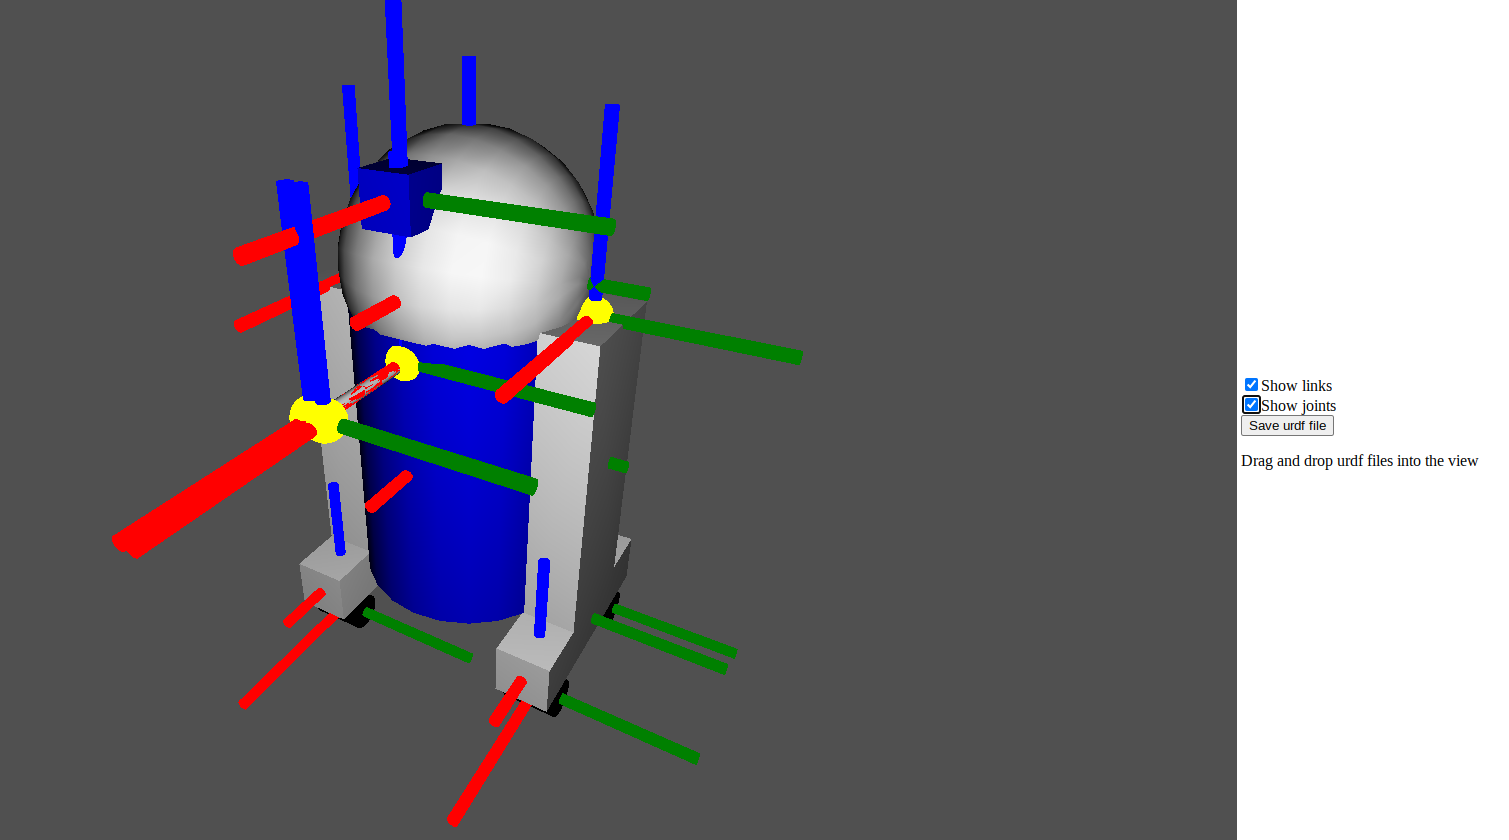
\includegraphics[width=0.85\linewidth]{Images/11_r2d2URDF.png}
        \caption{URDF editor by \href{https://github.com/danidask}{Dani Dask}}
        \label{fig:r2d2}
    \end{figure}

    \begin{figure}[H]
        \centering
        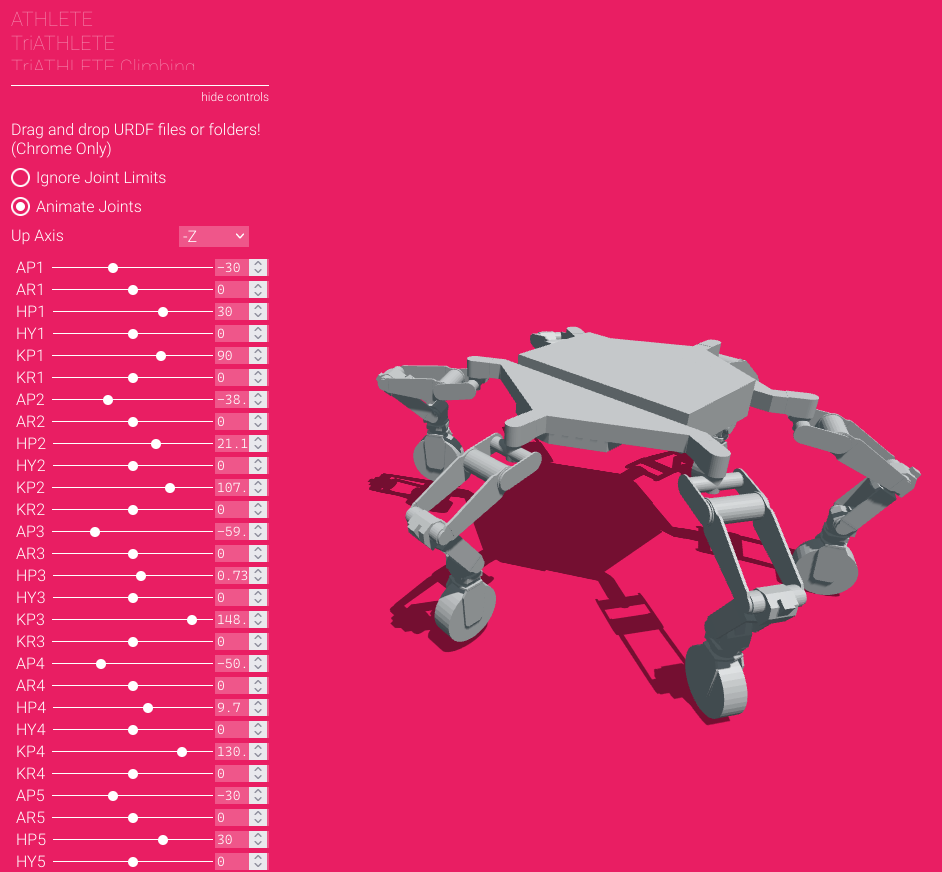
\includegraphics[width=0.85\linewidth]{Images/11_johnsonURDF.png}
        \caption{URDF loader by \href{https://github.com/gkjohnson}{Garrett Johnson}}
        \label{fig:johnsonURDF}
    \end{figure}

\section{JROS Profile}

    More time was dedicated this week to figuring out the issue with the ROS master in the Docker container. By modifying the extension's source code inside the container, the root cause of the issue was again identified as the base environment not being activated when JupyterLab is launched. This meant that none of the commands (\texttt{conda activate}, \texttt{mamba activate}, nor \texttt{micromamba activate}) in the \texttt{activate\_env.sh} script had any effect in activating the environment. As mentioned in Week 09, this problem is related to \href{https://github.com/conda/conda/issues/7980}{conda issue \#7980}. By using the workaround below in the startup scripts, the ROS master was able to successfully run in the Docker container.

    \begin{lstlisting}
# activate_env.sh
# Instead of using conda, mamba, or micromamba
source activate base
    \end{lstlisting}

    \noindent In spite of that, the ROS master can still not run in the JupyterHub environment. This can perhaps be an indicator that some of the configuration of the Docker image is being overwritten during the building process of the JROS profile. Further investigation is required.

\section{Future Work}

    The next big step in the project is to display the URDF loader in the widget tab of the extension. Once this is accomplished, it will need to be tested to ensure it dynamically responds to changes in the URDF. Lastly, the visual aspects of the extension such as layout and appearance will need to be assessed.

